\documentclass[12pt]{article}

% Layout.
\usepackage[top=1in, bottom=0.75in, left=1in, right=1in, headheight=1in, headsep=6pt]{geometry}

% Fonts.
\usepackage{mathptmx}
\usepackage[scaled=0.86]{helvet}
\renewcommand{\emph}[1]{\textsf{\textbf{#1}}}

% TiKZ.
\usepackage{tikz, pgfplots,xcolor}

\usetikzlibrary{calc,trees,positioning,arrows,fit,shapes,through, backgrounds}
\usetikzlibrary{patterns}

\usetikzlibrary{decorations.markings}
\usetikzlibrary{arrows}

\usepackage{pgfplots}


% Misc packages.
\usepackage{amsmath,amssymb,latexsym}
\usepackage{graphicx}
\usepackage{array}
\usepackage{xcolor}
\usepackage{multicol}
\usepackage{fancyhdr}
\pagestyle{fancy}


% Misc.
\renewcommand{\d}{\displaystyle}
\newcommand{\ds}{\displaystyle}
\newcommand{\ul}[1]{\underline{#1}}
\def\bc{\begin{center}}
\def\ec{\end{center}}
\def\be{\begin{enumerate}}
\def\ee{\end{enumerate}}

\newcommand{\ans}[1][1in]{\rule{#1}{.5pt}}


\lhead{Math F113X: Quiz 6}
\rhead{March 21, 2025}

\begin{document}

\vspace{1cm}
\strut

\noindent \textbf{Name:} \hrulefill \quad  score:\ans[1cm] \ / 10 \\


\noindent There are 10 points possible on this quiz. No aids (book, notes, etc.)
are permitted. You may use a calculator.  {\bf Show all work and supporting calculations for full credit. Explain how you get your answers.}

Questions 1 and 2 will use the weighted graph below. Edges weights are written in the middle of each edge and in the table to the right.

\begin{minipage}{0.4\textwidth}
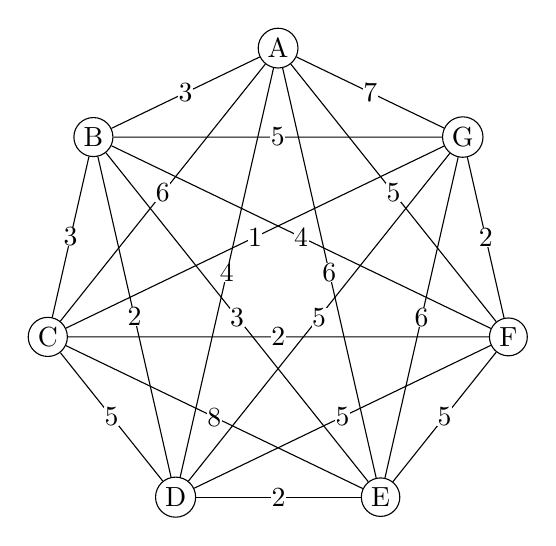
\begin{tikzpicture}[vtx/.style={draw, circle, inner sep =1.5 pt}, lbl/.style =  {inner sep =0.2 pt, fill = white}]
\foreach \i/\j in {0/A,1/B,2/C,3/D,4/E,5/F,6/G}{\node[vtx] (\i) at (360*\i/7+90:3){\j};}
%edges for 6 or G
\foreach \i/\j in {0/7,1/5,2/1,3/5,4/6,5/2}{\draw (6) -- node[lbl] {\j} (\i);}
%edges for 5 or F
\foreach \i/\j in {0/5,1/4,2/2,3/5,4/5}{\draw (5) -- node[lbl] {\j} (\i);}
%edges for 4 or E
\foreach \i/\j in {0/6,1/3,2/8,3/2}{\draw (4) -- node[lbl] {\j} (\i);}
%edges for 3 or D
\foreach \i/\j in {0/4,1/2,2/5}{\draw (3) -- node[lbl] {\j} (\i);}
%edges for 2 or C
\foreach \i/\j in {0/6,1/3}{\draw (2) -- node[lbl] {\j} (\i);}
%edges for 1 or B
\foreach \i/\j in {0/3}{\draw (1) -- node[lbl] {\j} (\i);}
\end{tikzpicture}
\end{minipage}
\begin{tabular}{c||c|c|c|c|c|c|c}
&A&B&C&D&E&F&G\\
\hline \hline 
A&0&3&6&4&6&5&7\\
B&3&0&3&2&3&4&5\\
C&6&3&0&5&8&2&1\\
D&4&2&5&0&2&5&5\\
E&6&3&8&2&0&5&6\\
F&5&4&2&5&5&0&2\\
G&7&5&1&5&6&2&0\\
\end{tabular}



\be

\item (4 points) Use the Nearest Neighbor Algorithm (NNA) starting at vertex $G$ to find a Hamiltonian circuit in the graph. Draw the circuit on the vertices below and determine weight of the circuit.\\

\textbf{Nearest Neighbor Algorithm:} From the present vertex, move to the nearest \emph{unvisited} vertex until all vertices are visited. Then close the circuit.\\

\begin{tikzpicture}[scale=.7,vtx/.style={draw, circle, inner sep =1.5 pt}, lbl/.style =  {inner sep =0.2 pt, fill = white}]
\foreach \i/\j in {0/A,1/B,2/C,3/D,4/E,5/F,6/G}{\node[vtx] (\i) at (360*\i/7+90:3){\j};}
\end{tikzpicture}
\hfill circuit weight: \underline{\hspace{2in}}.


\newpage
\begin{minipage}{0.4\textwidth}
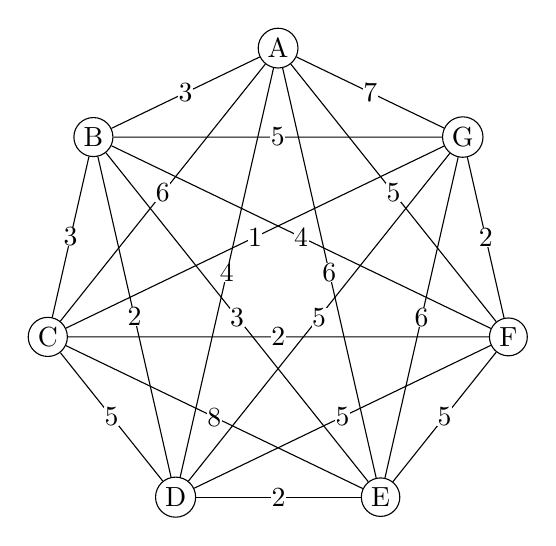
\begin{tikzpicture}[vtx/.style={draw, circle, inner sep =1.5 pt}, lbl/.style =  {inner sep =0.2 pt, fill = white}]
\foreach \i/\j in {0/A,1/B,2/C,3/D,4/E,5/F,6/G}{\node[vtx] (\i) at (360*\i/7+90:3){\j};}
%edges for 6 or G
\foreach \i/\j in {0/7,1/5,2/1,3/5,4/6,5/2}{\draw (6) -- node[lbl] {\j} (\i);}
%edges for 5 or F
\foreach \i/\j in {0/5,1/4,2/2,3/5,4/5}{\draw (5) -- node[lbl] {\j} (\i);}
%edges for 4 or E
\foreach \i/\j in {0/6,1/3,2/8,3/2}{\draw (4) -- node[lbl] {\j} (\i);}
%edges for 3 or D
\foreach \i/\j in {0/4,1/2,2/5}{\draw (3) -- node[lbl] {\j} (\i);}
%edges for 2 or C
\foreach \i/\j in {0/6,1/3}{\draw (2) -- node[lbl] {\j} (\i);}
%edges for 1 or B
\foreach \i/\j in {0/3}{\draw (1) -- node[lbl] {\j} (\i);}
\end{tikzpicture}
\end{minipage}
\begin{tabular}{c|c||c|c||c|c|}
edge&weight&edge&weight&edge&weight\\
\hline \hline 
CG&1&BE&3&DG&5\\
BD&2&AD&4&EF&5\\
CF&2&BF&4&AC&6\\
DE&2&AF&5&AE&6\\
FG&2&BG&5&EG&6\\
AB&3&CD&5&AG&7\\
BC&3&DF&5&CE&8\\
\end{tabular}


\item (4 points) Use the Cheapest Link Algorithm to find a Hamiltonian circuit in the graph (drawn above). Draw the circuit on the vertices below and determine weight of the circuit. \\

\textbf{Cheapest Link Algorithm:} Select the cheapest edge in the graph that does not create a vertex of degree 3 or close the circuit too soon.\\

\begin{tikzpicture}[scale=.7,vtx/.style={draw, circle, inner sep =1.5 pt}, lbl/.style =  {inner sep =0.2 pt, fill = white}]
\foreach \i/\j in {0/A,1/B,2/C,3/D,4/E,5/F,6/G}{\node[vtx] (\i) at (360*\i/7+90:3){\j};}
\end{tikzpicture}
\vfill
\hfill circuit weight: \underline{\hspace{2in}}.
\item (1 point) How many different Hamiltonian circuits does a graph on 7 vertices have? (It is sufficient to indicate how it is computed.)
\vfill
\item (1 point) Is either algorithm, NNA or the Cheapest Link, \emph{guaranteed} to give the cheapest Hamiltonian circuit in \emph{every} graph? Explain your answer. 
\vfill
 \ee
\end{document}